\section{Second Member}
This is the section dedicated to one of the team members, and it should be written individually . It can include a range of things; first subsection is a space for you to point out the strengths and weaknesses of the module, including complaints about the module coordinator Max Wilson. The second section should have a selfie image with Max! The last part of it is the most important one. You will need to write a paragraph about what you have learned in this module. You can write it in \textbf{Bold} if you want or you can use other fonts. 

Please do not forget:
\begin{itemize}
	\item First paragraph should have your comments about the module
	\item Second one, a selfie img with Max
	\item Last one, what you learned in this module.
\end{itemize}

\subsection{Comments about the module}
So far the module has been a good way of getting an overview of the whole software engineering process and the work that it includes beyond the coding. It has been helpful to see why all of these things are important and the real-life examples provided in lectures and extra reading has been helpful. 

\subsection{Selfie with Max}
\begin{figure}[h]
\caption{Selfie with Max}
\centering
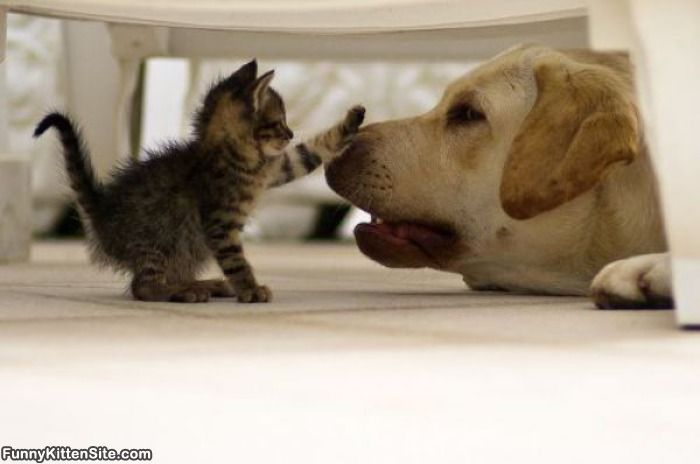
\includegraphics[width=0.5\textwidth]{download}
\label{fig:selfie}
\end{figure}


My selfie with Max is in  Figure~\ref{fig:selfie}.

\subsection{What I have learned in this module}
I have learnt UML and why it is important to focus on requirements and specifications before you start to develop a system. 

